\chapter{Introduction}
\label{ch:introduction}

\def\figdir{chapters/introduction/figures/}

%\epigraph{\textit{The easiest way to solve a problem is to deny it exists.}}{Isaac Asimov}

%\begin{quote} 
%	\begin{flushright}
%		\textit{The easiest way to solve a problem\\ is to deny it exists.}
%		
%		--- ~ Prof. Isaac Asimov
%	\end{flushright}
%\end{quote}

\section{Motivation}

\lettrine[lines=3,nindent=0em,loversize=0.1]{T}{he} global population is steady rising and migrating from rural areas to urban areas and results in a growing urbanization as urban for past two centuries. This result of a rapid rise in urban population and therefore in future the ecology of the urban system will become a primary concern. Furthermore, climate change, driven by human activity need to be reduces to mitigate the present detrimental climatology in urban areas. A lack thereof can not only have implication on the global climate but also the comfort and health of urban populace. 

Presently, there is a growing need to accurately predict the impact of the vegetation. Vegetation provides natural cooling through shading and transpiration and is a primary solution to combat the growing urban heat island (UHI) and improve the thermal comfort  \citep{Gillner2015, Bowler2010, Loughner2012}. 


\section{Objective and Methodology}

The objective of this thesis is as follows:
\begin{itemize}
	\item to quantify the natural cooling provided by vegetation in urban microclimate consisting of transpirative cooling and shading from plant foliage.
	\item to quantify the impact of vegetation on pedestrian thermal comfort. 
	\item to understand the influence of water stress on the natural cooling.
\end{itemize}

Figure \ref{fig:vegetation_fluxes} shows a schematic representation of the various fluxes exchanged between an urban tree and the environment. 

\begin{figure}[h]
	\centering
	%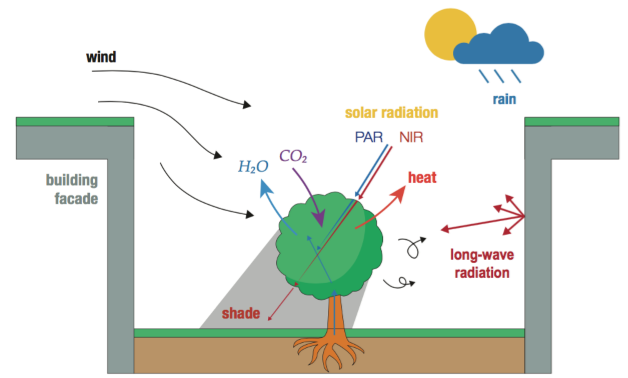
\includegraphics[width=0.7\textwidth]{\figdir/vegetation_fluxes.png}
	\caption{Interaction of urban vegetation with the urban microclimate.}
	\label{fig:vegetation_fluxes}
\end{figure}	



\section{Outline of the thesis}

The 